\chapter{Autoencoders}
The idea of autoencoders is that we want to force a network to try to reconstruct our data and hopefully it will learn a useful representation of the data. For traditional autoencoders this is use for feature learning and for variational atoencoders to generate fake samples.

\section{Traditional Autoencoder}
\begin{figure}[!htb]
  \centering
  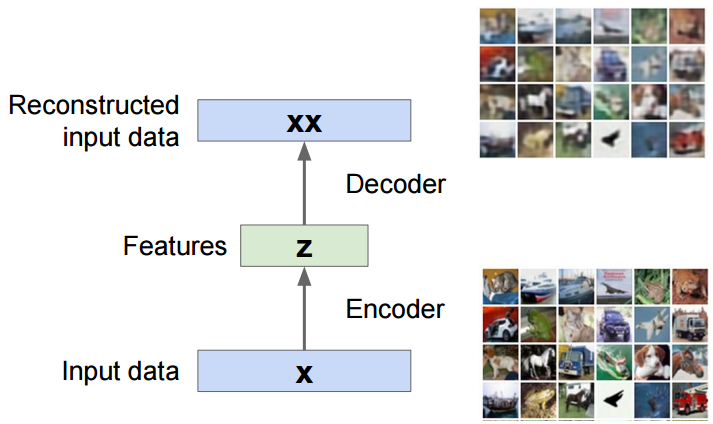
\includegraphics[width=0.45\textwidth]{Images/autoencoders/1.png}
  \caption{Traditional Autoencoder}
\end{figure}

Normally encoder will be a 4-layer conv, and the decoder a 4-layer upconv. Sometimes they share weights (in fact they are the same, we only have to transpose them): $\dim(x) = D, \dim(z)=H$, $w_e : H \times D, w_d : D \times H = w_e^T$.

The idea is to pass the input data through an encoder network that will produce features $z$. This step can be thought as PCA. We are transforming the input data and transforming it into another feature representation. The encoder network is usually a ReLU CNN. Normally $z$ is smaller than $x$ (dimensionality reduction).

The problem is that we do not have any explicit labels to use to know which information is relevant and which one its not to decide how to make the dimensionality reduction. To decide which is the most relevant data we reconstruct the input data only with the information in the $z$ features and compare the reconstruction with the original image.

Specially if the $z$ features are small, hopefully, it will force the network to summarize the useful statistics and to discover useful features of the input image.



\subsection*{How do we train them?}
\begin{figure}[!htb]
  \centering
  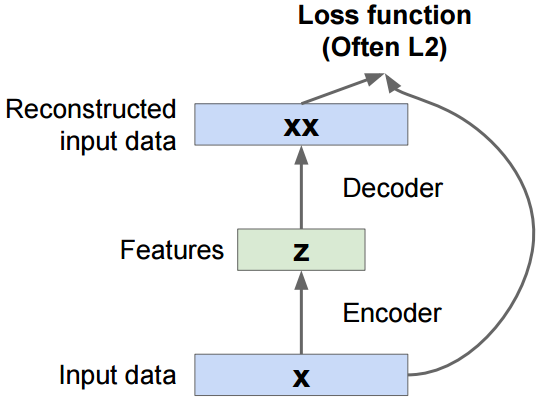
\includegraphics[width=0.35\textwidth]{Images/autoencoders/2.png}
  \caption{Traditional Autoencoder}
\end{figure}
Normally it is trained as a regular NN with euclidean distance as the loss function comparing the input data vs the reconstructed data. 

Normally, after training, the decoder will be thrown away.


\subsection*{Unsupervised + Supervised learning}
\begin{figure}[!htb]
  \centering
  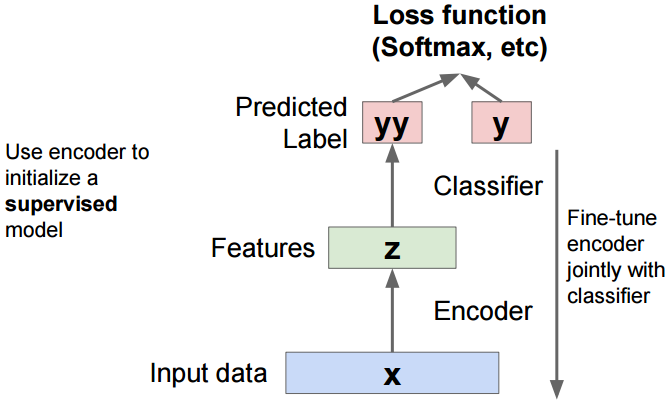
\includegraphics[width=0.4\textwidth]{Images/autoencoders/3.png}
  \caption{Traditional Autoencoder}
\end{figure}
The idea is first to train the network with unsupervised data, and then fine tune with a small labeled dataset. This idea is beautiful in the sense that we could train our networks with millions of unlabeled data from the internet, and the fine tune the network with a labeled dataset such us KITTI. The problem is that is yet not working that well.

\section{Variational Autoencoder}
Transforming traditional autoencoders to Bayesian, allows us to generate data.

\begin{figure}[!htb]
  \centering
  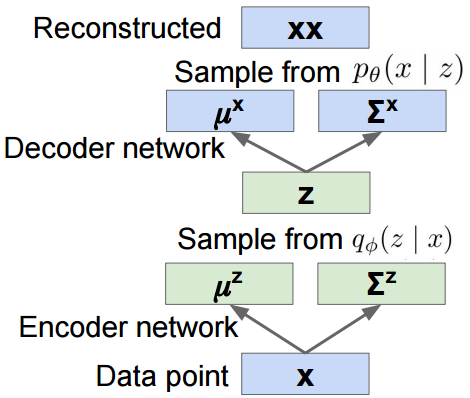
\includegraphics[width=0.3\textwidth]{Images/autoencoders/4.png}
  \caption{Variational Autoencoder}
\end{figure}

We assume that it exists a distribution with parameters $\phi^*$ that is generating the latent states $z$ from $x$ (given $x$ we can sample $z$): $q_{\phi^*}(z|x)$

We also assume a conditional distribution with parameters $\theta^*$ that given the latent states we can sample $x$: $p_{\theta^*}(x|z^{(i)})$

We assume that these distributions are diagonal Gaussian and we will try to approximate them with two neural nets with parameters $\phi$ and $\theta$. Also, we assume $p_{\theta^*}(z)$ unit Gaussian. We could assume more fancy distributions, but we use these ones because they are easy to work with.

\begin{enumerate}
\item Input data $x$
\item Pass $x$ through the encoder network which will spit out a distribution of the latent states $z$ ( the mean and (diagonal) covariance of $q_{\phi}(z|x)$).
\item Sample latent states of high probability from the obtained distribution $q_{\phi}(z|x)$ given our input data $x$.
\item Once we have some samples of $z$, pass them trough the decoder which will spit out the distribution of the input data $x$ ( the mean and (diagonal) covariance of $p_{\theta^*}(x|z^{(i)})$)
\item Finally, we can sample data $xx$ of high probability from the obtained distribution $p_{\theta}(x|z)$ given the latent variables $z$. $xx$ should be similar to $x$.
\end{enumerate}

\subsection*{Generate fake data}
We train Variational Autoencoders as a normal autoencoder: reconstruction loss at the end, regularization toward prior in the middle. After the network is trained we can use it to generate fake data.

\begin{enumerate}
\item We first sample from the prior distribution $p_{\theta}(z)$ which we have assumed that it is unit Gaussian so it is really easy to draw random samples from this distribution.
\item Pass a sample through the decoder network which we have trained during tinning. The decoder will spit out a distribution over our data points x in terms of both a mean and covariance
\item Once we have a mean and a covariance, we have a the $p_{\theta}(x|z)$ which is also easy to sample from because we have assume that is diagonal Gaussian. This samples are going to be new fake data $xx$
\end{enumerate}

\begin{figure}[!htb]
  \centering
  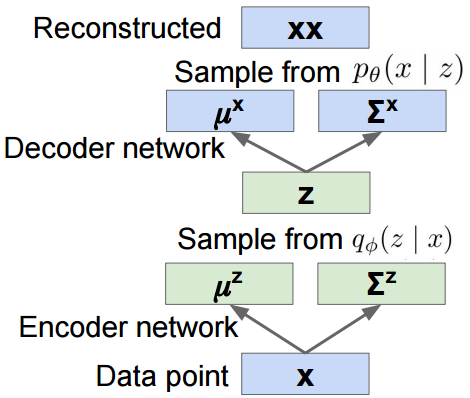
\includegraphics[width=0.3\textwidth]{Images/autoencoders/4.png}
  \caption{Generate data with Variational Autoencoder}
\end{figure}

To try figuring out what the decoder network has learn we can densely sample all the latent space.

\begin{figure}[!htb]
  \centering
  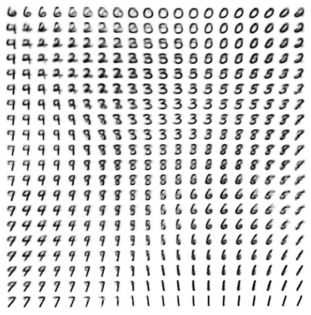
\includegraphics[width=0.3\textwidth]{Images/autoencoders/6.png}
  \caption{In this example, the encoder was trained with a latent space of two dimensions. This image was generated by passing each point of this 2D latent space through the decoder. It can be seen that the net has learn to interpolate the digits. For example, we can see 6s transforming to 0s.}
\end{figure}


One of the reasons that is making this nice separation of classes between axes, is that we are assuming diagonal distribution. Thus, we are assuming as a prior to our system that latent variables (axis in the latent space) are independent (there is no relation between them).

\begin{figure}[!htb]
  \centering
  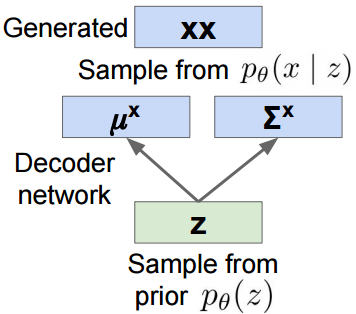
\includegraphics[width=0.25\textwidth]{Images/autoencoders/5.png}
  \caption{Example of dense sampling of the latent space}
\end{figure}

In the CS231n course - lecture 14 there is more information explaining that it is not possible to use maximum likelihood and explaining how to solve this situation.

\subsection*{All together}
A recent paper (Dosovitskiy and Brox, “Generating Images with Perceptual Similarity Metrics based on Deep Networks”, arXiv 2016) proposes a method to mix all together to make the fake images more realistic.
\begin{figure}[!htb]
  \centering
  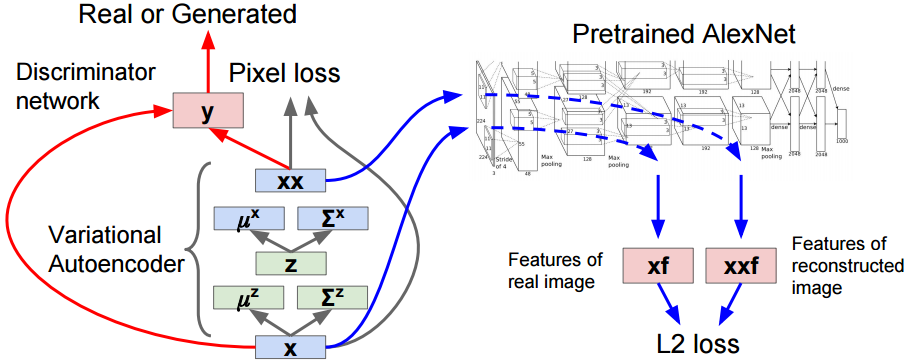
\includegraphics[width=0.6\textwidth]{Images/autoencoders/11.png}
  \caption{All together to generate better images}
\end{figure}

\section*{Overview}
The idea of autoencoders is that we want to force a network to try to reconstruct our data and hopefully it will learn a useful representation of the data. For traditional autoencoders this is use for feature learning and for variational atoencoders to generate fake samples.

\begin{itemize}
\item Traditional Autoencoders
\begin{itemize}
\item Try to reconstruct input
\item Used to learn features, initialize supervised model
\item Not used much anymore
\end{itemize}
\item Variational Autoencoders
\begin{itemize}
\item Bayesian meets deep learning
\item Sample from model to generate images
\end{itemize}
\end{itemize}
